\chapter{Kravspecifikation}\label{ch:Krav}

I projektet er user stories blevet benyttet til at beskrive den ønskede funktionalitet for systemet. Disse user stories er lavet på baggrund af MoSCoW-analysen fra afsnit \ref{ch:Moscow}.
De enkelte user stories er blevet samlet til en række af epics, der viser systemets overordnede funktionalitet. Disse epics vises på aktør-kontekst diagrammet, der ses på figur \ref{fig:KontekstDia}. 

\begin{figure}[H]
	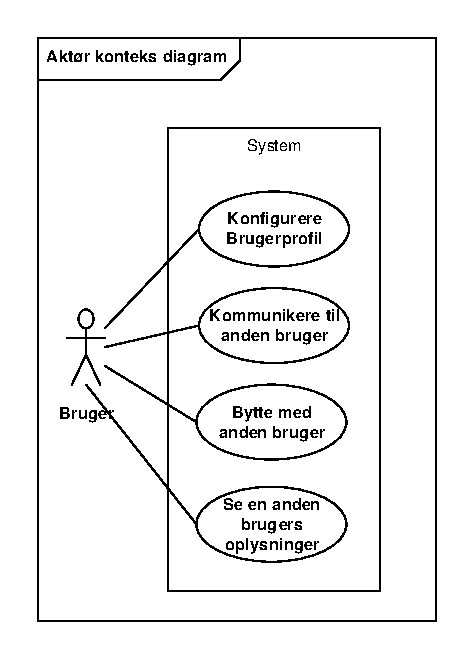
\includegraphics[width=140mm,height=150mm]{../Dokumentation/figures/KontekstDiagram.PDF}
	\caption{Aktør-kontekst diagram for BargainBarter}
	\label{fig:KontekstDia}
\end{figure}

\noindent Igennem rapporten vil der bliver fokuseret på følgende to user stories: ''Oprette en bytteannonce'' og ''Søg efter bytteannoncer''. Der gås i dybden med disse to user stories, da de er blandt de mest centrale, og da de eksemplificerer den generelle virkemåde af systemet.\\

 For den fulde liste og beskrivelse af de udarbejde user stories for systemet henvises til dokumentationen\footnote{Se bilag - Dokumentation, sektion 3}.\\
De to udvalgte user stories kan læses nedenunder:

\section{Oprette en bytteannonce}
{\color{blue}\textbf{EGENSKAB}:} Oprette en bytteannonce \\
Som bruger \\
Ønsker jeg at kunne oprette en bytteannonce \\
For at kunne bytte med andre brugere af systemet.\\ \\
{\color{blue}\textbf{BAGGRUND}} \\
{\color{blue}\textbf{Givet}} at bruger er logget ind \\ \\
{\color{blue}\textbf{SCENARIE:}} Oprette en bytteannonce \\
{\color{blue}\textbf{Når}}  bruger ønsker at oprette en bytteannonce i systemet \\
{\color{blue}\textbf{Så}} navigerer han til menupunktet ”Opret annonce” \\
{\color{blue}\textbf{Så}} udfylder han bytteannonce-skabelonen \\
{\color{blue}\textbf{Og}} trykker på ”Opret annonce”-knappen
\section{Søg efter bytteannoncer}
{\color{blue}\textbf{EGENSKAB}:}Søg efter bytteannoncer \\
Som bruger \\
Ønsker jeg at kunne søge efter bytteannoncer \\
For at kunne finde en bestemt type vare\\ \\
{\color{blue}\textbf{BAGGRUND}} \\
{\color{blue}\textbf{Givet}} at bruger er logget ind \\
\\
{\color{blue}\textbf{SCENARIE:}} Søg efter bytteannoncer \\
{\color{blue}\textbf{Når}} bruger ønsker at søge efter bytteannoncer i systemet\\
{\color{blue}\textbf{Så}} navigerer brugeren til menupunktet ”Søg” \\
{\color{blue}\textbf{Så}} indtaster brugeren søgekriterier som består af(Kategori, afstand, evt byttegenstand)\\
{\color{blue}\textbf{Og}} trykker på “søg“-knappen

\section{Ikke-funktionelle krav}
I forbindelse med udarbejdelsen af systemet er der blevet fastsat nogle ikke-funktionelle krav til systemet. De ikke-funktionelle krav omhandler primært performance, brugervenlighed og skalerbarhed.\\ For en liste over de specifikke krav henvises til dokumentationen\footnote{Se bilag - Dokumentation, sektion 4}
